\documentclass[12pt]{article}
\usepackage[latin1]{inputenc}
\usepackage[english]{babel}
\usepackage{amsmath}
\usepackage{amssymb}
%\usepackage{dsfont}
\usepackage{theorem}
\usepackage{graphicx}
\usepackage{hyperref}
\usepackage{lscape}
\usepackage{enumerate}
\usepackage{verbatim}
\usepackage{float}
\usepackage{fancyhdr}
%\usepackage{bigints}
\pagestyle{fancy}

\newtheorem{theorem}{Theorem}[section]
\newtheorem{lemma}[theorem]{Lemma}
\newtheorem{proposition}[theorem]{Proposition}
\newtheorem{corollary}[theorem]{Corollary}

\newenvironment{proof}[1][Proof:]{\begin{trivlist}
\item[\hskip \labelsep {\bfseries #1}]}{\end{trivlist}}
\newenvironment{definition}[1][Definition:]{\begin{trivlist}
\item[\hskip \labelsep {\bfseries #1}]}{\end{trivlist}}
\newenvironment{example}[1][Example:]{\begin{trivlist}
\item[\hskip \labelsep {\bfseries #1}]}{\end{trivlist}}
\newenvironment{remark}[1][Remark:]{\begin{trivlist}
\item[\hskip \labelsep {\bfseries #1}]}{\end{trivlist}}

\newcommand{\qed}{\nobreak \ifvmode \relax \else
      \ifdim\lastskip<1.5em \hskip-\lastskip
      \hskip1.5em plus0em minus0.5em \fi \nobreak
      \vrule height0.75em width0.5em depth0.25em\fi}

\newcommand*{\QEDA}{\hfill\ensuremath{\blacksquare}}
\newcommand*{\QEDB}{\hfill\ensuremath{\square}}

\newcommand{\dif}{\mbox{d}}


%---------------------------------
%\topmargin -.5 in
%\textheight 22 cm
%\textwidth 16 cm
%\oddsidemargin 0 cm
%\evensidemargin 0 cm
%---------------------------------


\title{Growing Degree Days in Canada - Data Project}
\author{A. Naveen, C. Chagas, A. Iyer, O. Abramov, E. Kielley, R. Brecht}
\date{\today}

\begin{document}

\maketitle
\vspace{5pt}
\tableofcontents
\vspace{40pt}

\section{Motivation}
We want to use Python and Bash scripts to analyse growing degree days (GDD) for three different cities in Canada. Growing degree days are used to predict when a flower or plant will bloom. 
\\ Plants require energy to grow and develop, and some of this energy is in the form of heat. The heat required is expressed as degrees of temperature. Temperature regulates many of the physical and chemical processes within a plant, which in turn control the rate of growth and development toward maturity. 
\\The amount of heat accumulated during the day, as obtained by subtracting the plant's base temperature from the mean temperature for the day, is termed the degree-day accumulation.
\\


\pagebreak
\section{Minimum core tasks}

\subsection{Files and Scripts}
\begin{description}
\item[gdd.py]
\item Input: tbase, tupper, input\_folder (optional)
\item Output: year\_cityName\_tbase\_tupper\_gdd.csv
\item Searches for files that ends with \emph{temp.csv}. We expect, that these
files have the columns: Date/Time, Min Temp(${}^\circ$C), Max Temp(${}^\circ$C).

Then these columns of each file will be copied into a new csv file with the name
\emph{year\_cityName\_tbase\_tupper\_gdd.csv}, where cityName is extracted of the
current file name. That file will be saved in the folder \emph{Output}.
After that, a column called GDD will be added. The value of
cell $n$ is calculated with the formula:
$$
\sum_{i=1}^n \big( \tfrac{\text{tmax}_i+\text{tmin}_i}{2}-\text{tbase}\big)
$$
If $\text{tmax}_i$ or $\text{tmax}_i$ is bigger than tupper it is set to tupper,
 also if $\text{tmin}_i$ or $\text{tmax}_i$ 
is  smaller than tbase then it is set to tbase.

%\item[gdd.sh]
%\item Input: temperatures.csv, tbase, tupper
%\item Output:
%\item What it does... maybe adding code

\item[create\_plots.py]
\item Output: CumulativeGDD.png, CompareMaxMinTemp.png
\item Searches for files ending with \emph{gdd.csv}. 
Then reads of each file the max and min temperature column and creatas a subplot
showing the time line of the max and min temperature. Also reads the GDD column 
and adds accumulated GDD to another figure. Finally saves the two created figures
 as PNG-files in the \emph{Plot} folder.

\end{description}
\subsection{Process flow}
The following diagramm shows the dependencies and execution steps of the scripts
we are running.
\\~\\
By executing the \emph{Makefile}, we create a folder called \emph{Output} and run
the python script \emph{gdd.py} with the arguments tbase=10, tupper=30 and the path
 \emph{./Input/}. This produces 3 csv files, because we have 3 files of the 
format \emph{year\_cityName\_.csv} in the folder \emph{Input}.
Next the script \emph{create\_plots.py} is called by Makefile and produces 2 PNG-
files. Finally Makefile creates the file \emph{report.pdf} by compiling the 
\emph{report.tex} file.

	\begin{figure}[!htbp]
		\centering
		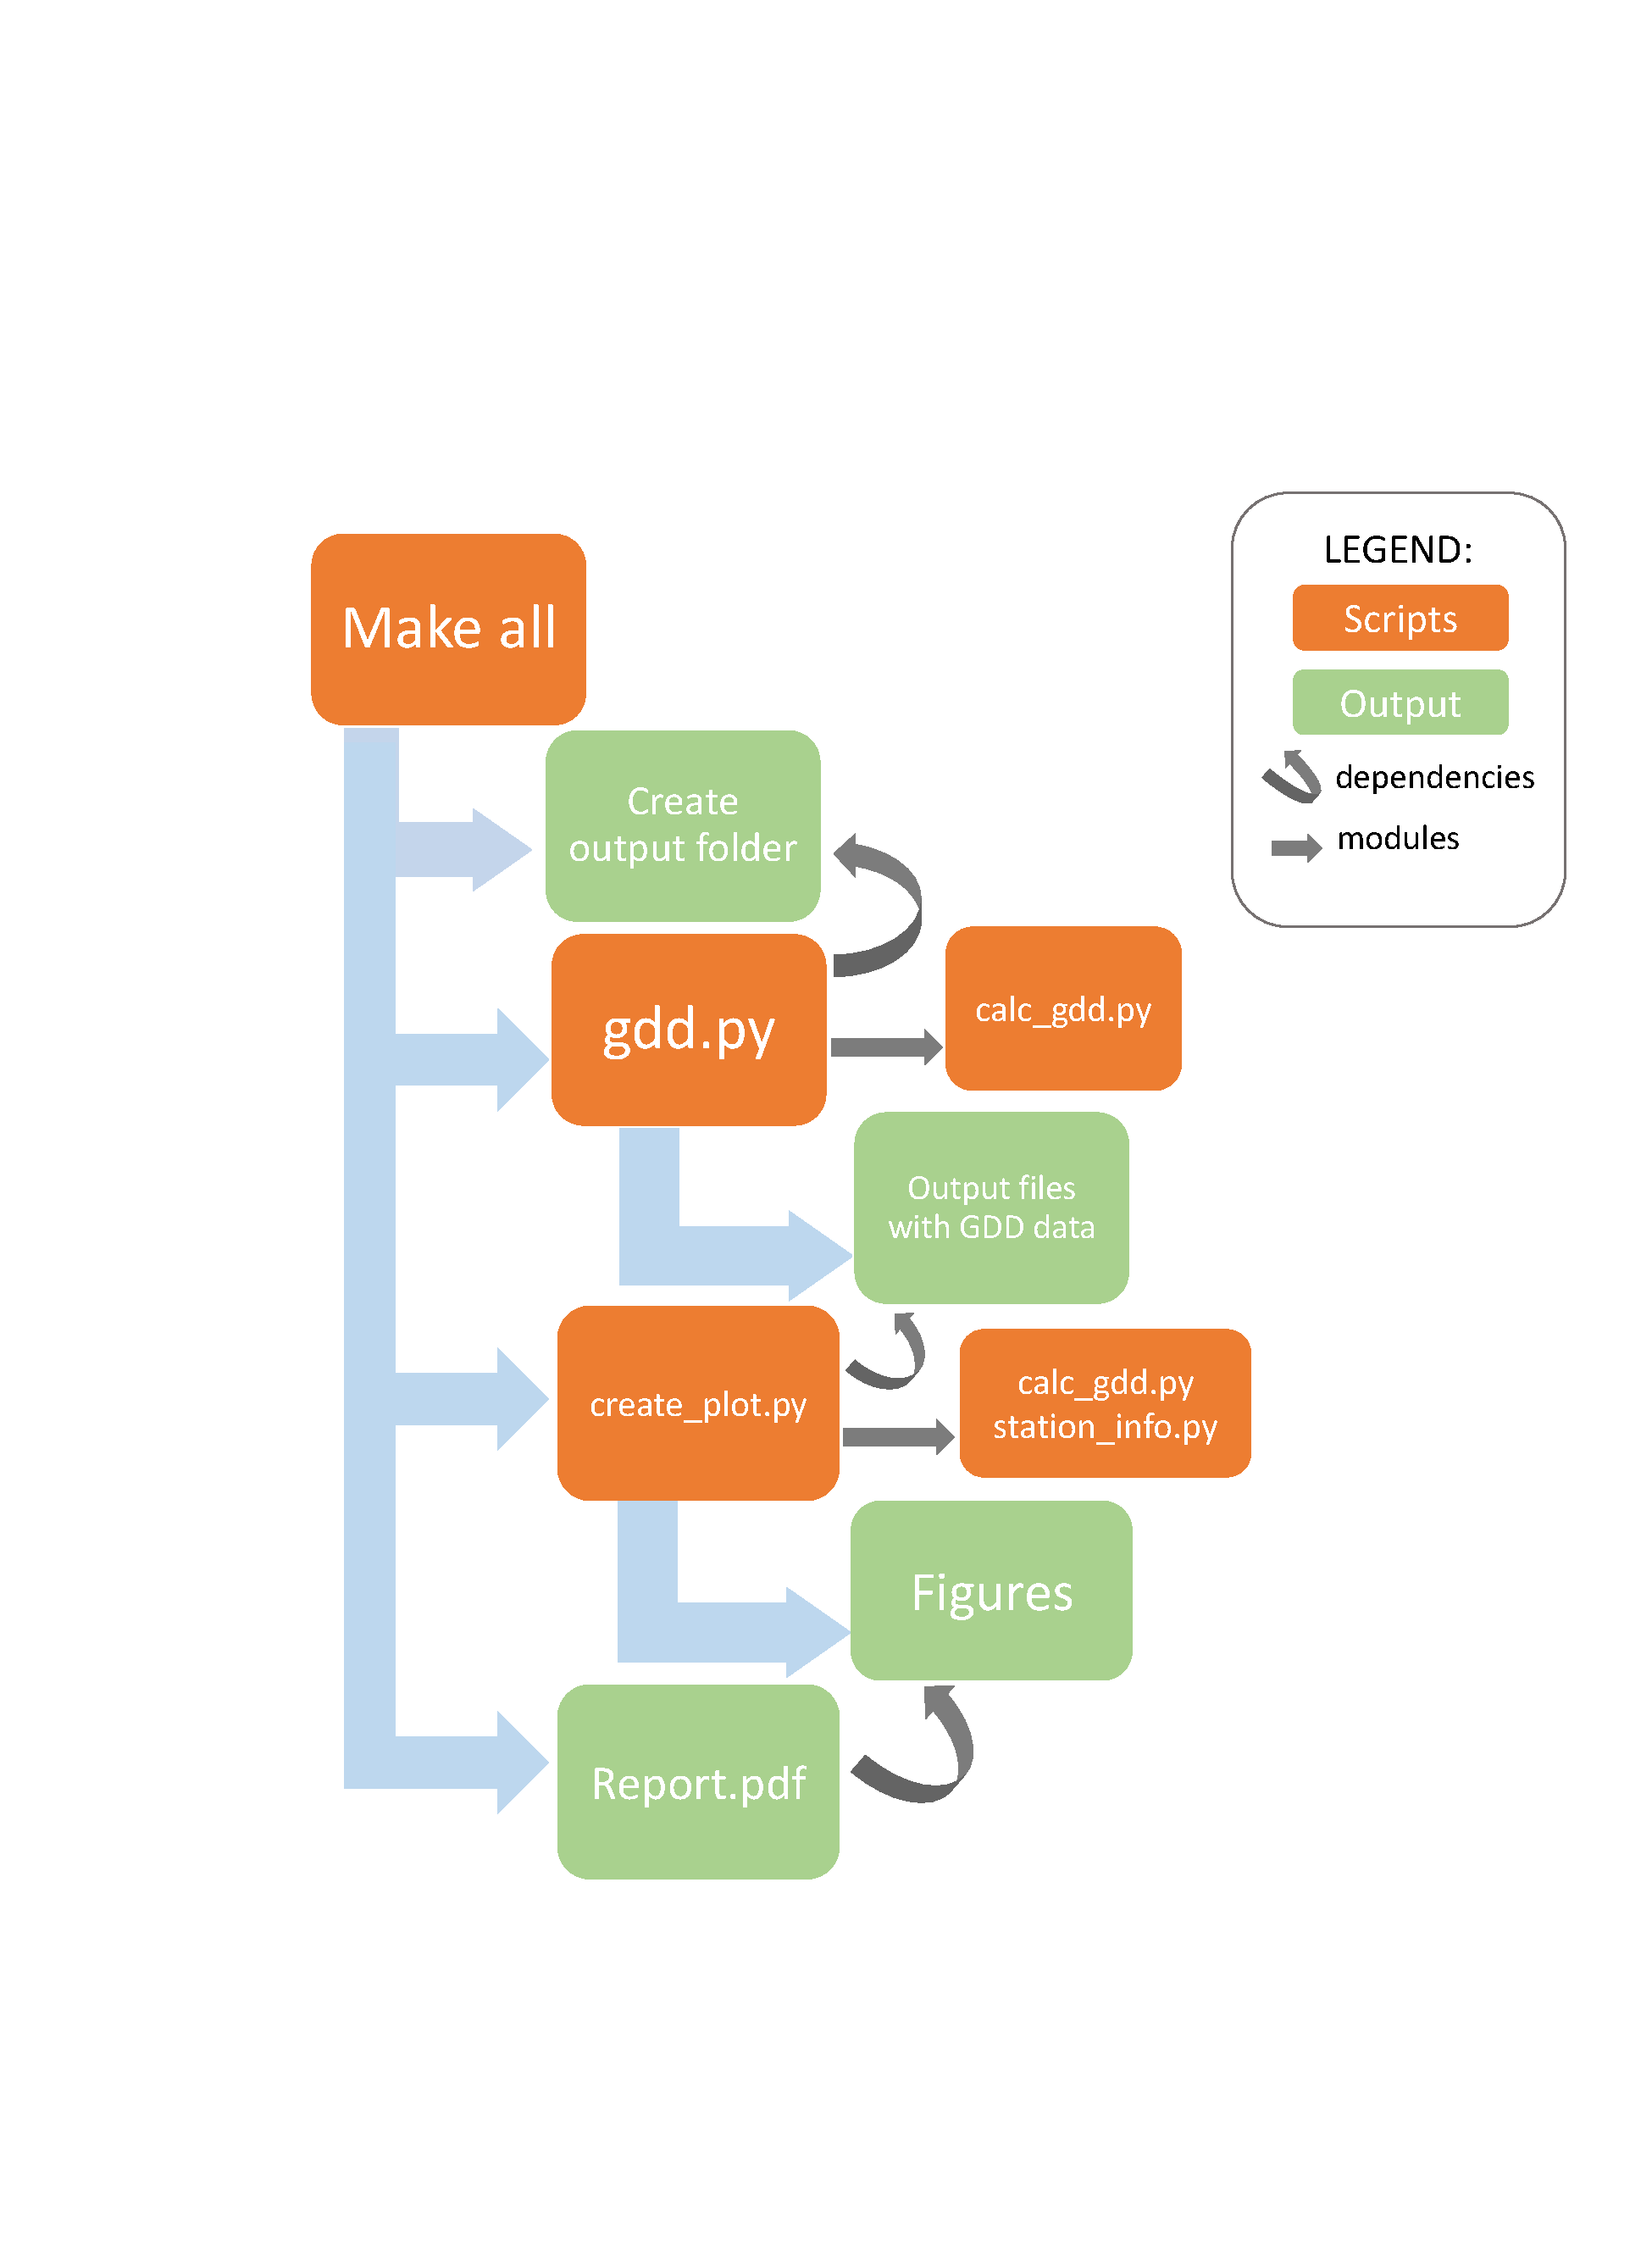
\includegraphics[width=0.9\textwidth]{./Report/diagram_workflow.pdf} 
		\caption{\scriptsize Shows the process flow of our scirpts.}\label{flowplot}		  
	\end{figure}


\pagebreak
\subsection{Results}
	\begin{figure}[!htbp]
		\centering
		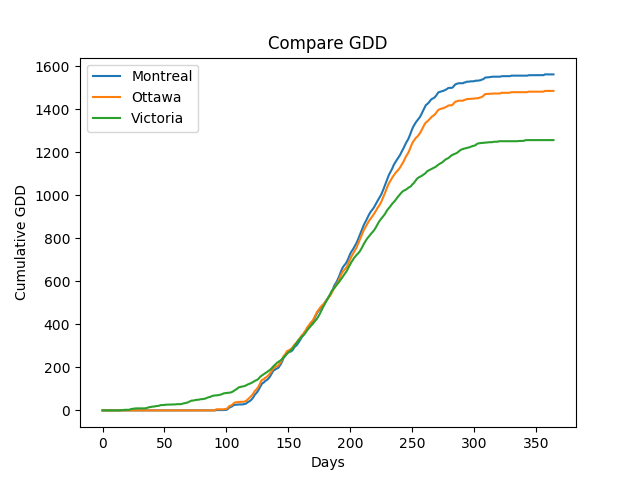
\includegraphics[width=0.9\textwidth]{./Output/CumulativeGDD.png} 
		\caption{\scriptsize Shows the accumulated GDD vs time for three selected cities.}\label{GDDplot}		  
	\end{figure}

	\begin{figure}[!htbp]
		\centering
		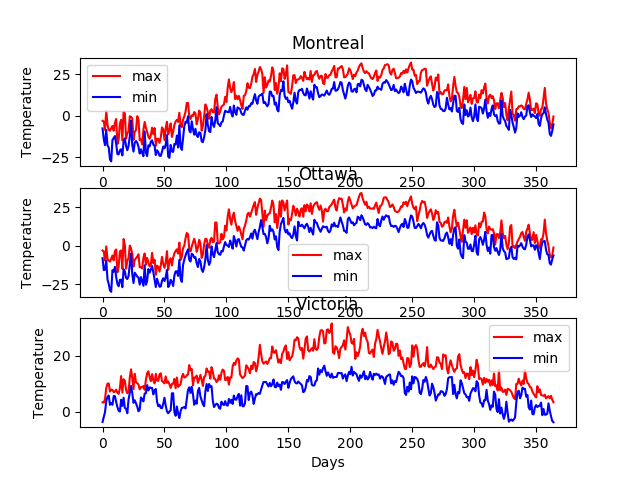
\includegraphics[width=0.9\textwidth]{./Output/CompareMaxMinTemp.png} 
		\caption{\scriptsize Shows the min and max temperature for three selected cities.}\label{MinMaxplot}		  
	\end{figure}

\pagebreak
\section{Secondary tasks}


\end{document}
